\documentclass[12pt, tikz, border=5mm]{standalone}
\usetikzlibrary{angles,
                quotes}
\usepackage{siunitx}

\begin{document}
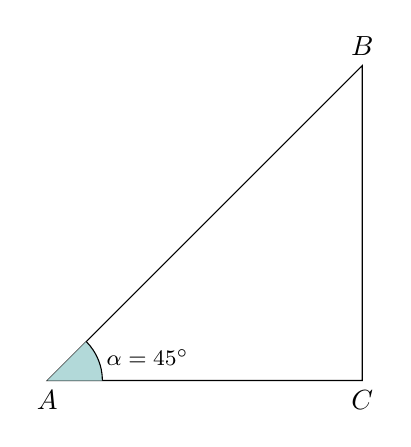
\begin{tikzpicture}[
my angle/.style = {draw, fill=teal!30,
                   angle radius=7mm, 
                   angle eccentricity=1.1, 
                   right, inner sep=1pt,
                   font=\footnotesize} 
                   ]
\draw   (0,0) coordinate[label=below:$A$] (a) --
            (4,0) coordinate[label=below:$C$] (c) --
            (4,4) coordinate[label=above:$B$] (b) -- cycle;
\pic[my angle, "$\alpha=\SI{45}{\degree}$"] {angle = c--a--b};

\end{tikzpicture}



\end{document}